\section{MTProto}

\subsection{Telegram}
Telegram è un applicativo di messaggistica istantanea rilasciato nel 2013 da Pavel Durov e Nikolai Durov.
Proponendosi come alternativa al popolarissimo WhatsApp, Telegram è riuscito a ritagliarsi una buona fetta di mercato,
raggiungendo proprio recentemente i 700 milioni di utenti (Giugno 2022). \\
I servizi offerti sono molti e comprendono le semplici chat, i gruppi di più utenti e i canali usati per il broadcast.
Telegram fornisce inoltre un'API di facile utilizzo per lo sviluppo di bot e script automatici in grado di interagire 
con il sistema. \\

Un altro aspetto particolarmente apprezzato, specialmente in alcuni ambiti, è la presunta sicurezza, privacy
e resistenza alla censura che questo social garantirebbe. \\
Alla base di tutto vi è un protocollo sviluppato da Telegram stesso, chiamato MTProto.

\subsection{Il protocollo MTProto}
\gls{mtproto} è un protocollo sviluppato da Telegram per la comunicazione sicura tra client e server. \\
La scelta di sviluppare un protocollo personalizzato invece che affidarsi a quelli già esistenti non è stata esente da critiche.
\gls{mtproto} è nato per affrontare alcune problematiche specifiche dell'ambito in cui opera:
\begin{itemize}
    \item garantire una certa affidabilità anche con le connessioni non all'altezza dei dispositivi mobili
    \item massimizzare la velocità nella gestione di grandi file, come foto e video
\end{itemize}

La prima versione di \gls{mtproto} presentava delle vulnerabilità che sono state evidenziate dal lavoro congiunto di due ricercatori dell'università di Aarhus \cite{inp:mtproto-v1-attacks}.
Sebbene nella pratica non si fosse riuscito ad individuare un attacco in grado di minare la sicurezza dei messaggi,
le criticità riscontrate nel protocollo sono state risolte con il rilascio della sua versione 2.0 nei client ufficiali v4.6 nel Dicembre del 2017 \cite{man:mtproto}. \\

Questa nuova versione ha superato diverse analisi volte a individuarne i punti deboli.
I risultati ne hanno comprovato la robustezza sia dal punto di vista crittografico \cite{inp:mtproto-attacks}
che dal punto di vista requisiti di sicurezza garantiti dal protocollo \cite{inp:mtproto-proverif}. \\

Va sottolineato inoltre che tutte le specifiche del protocollo sono pubbliche.
Ciò permette a chiunque di realizzare una propria versione del client in grado di interfacciarsi con tutti gli altri. \\

\gls{mtproto} è un protocollo piuttosto complesso, ed è composto da molteplici sotto-protocolli, ciascuno con un compito specifico.
Si va dall'autenticazione e lo scambio di chiavi fra client e server, alla creazione di chiavi di sessione fra due client
al fine di realizzare una cifratura end-to-end, giusto per citare alcune funzioni previste.

\subsection{}
\begin{figure}
    \centering
    % generated by Plantuml 1.2022.0       
    \definecolor{plantucolor0000}{RGB}{255,255,255}
    \definecolor{plantucolor0001}{RGB}{56,56,56}
    \definecolor{plantucolor0002}{RGB}{248,248,248}
    \definecolor{plantucolor0003}{RGB}{0,0,0}
    \definecolor{plantucolor0004}{RGB}{235,235,235}
    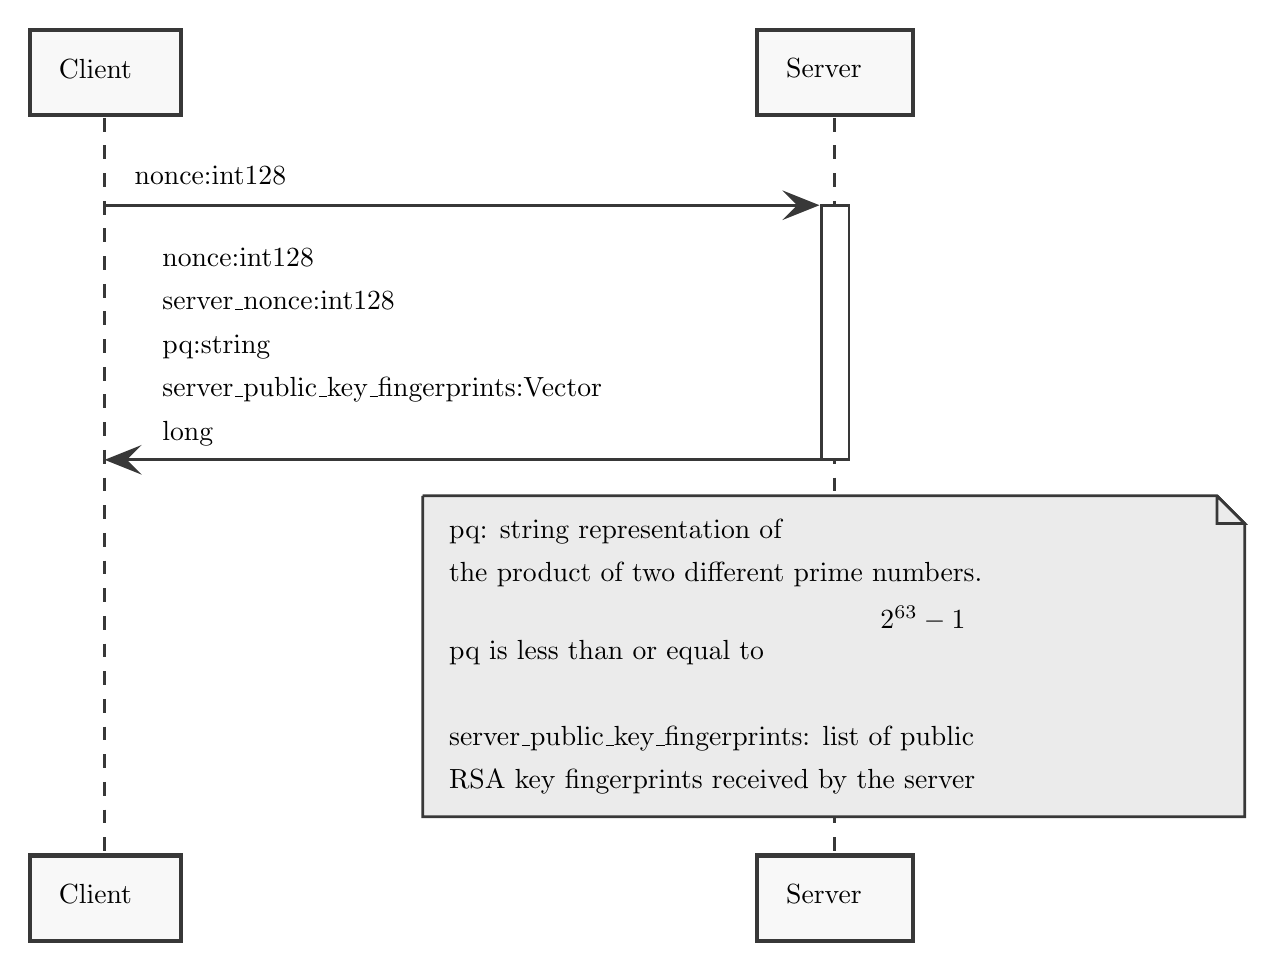
\begin{tikzpicture}[yscale=-1
            ,pstyle0/.style={color=plantucolor0001,fill=white,line width=1.0pt}
            ,pstyle1/.style={color=plantucolor0001,line width=1.0pt,dash pattern=on 5.0pt off 5.0pt}
            ,pstyle2/.style={color=plantucolor0001,fill=plantucolor0002,line width=1.5pt}
            ,pstyle3/.style={color=plantucolor0001,fill=plantucolor0001,line width=1.0pt}
            ,pstyle4/.style={color=plantucolor0001,line width=1.0pt}
            ,pstyle5/.style={color=plantucolor0001,fill=plantucolor0004,line width=1.0pt}
        ]
        \draw[pstyle0] (291.0218pt,68.3999pt) rectangle (301.0218pt,160.4pt);
        \draw[pstyle1] (32pt,36.7999pt) -- (32pt,304.4001pt);
        \draw[pstyle1] (295.7948pt,36.7999pt) -- (295.7948pt,304.4001pt);
        \draw[pstyle2] (5pt,5pt) rectangle (59.8pt,35.7999pt);
        \node at (12pt,12pt)[below right,color=black]{Client};
        \draw[pstyle2] (5pt,303.4001pt) rectangle (59.8pt,334.2pt);
        \node at (12pt,310.4001pt)[below right,color=black]{Client};
        \draw[pstyle2] (267.7948pt,5pt) rectangle (324.2488pt,35.7999pt);
        \node at (274.7948pt,12pt)[below right,color=black]{Server};
        \draw[pstyle2] (267.7948pt,303.4001pt) rectangle (324.2488pt,334.2pt);
        \node at (274.7948pt,310.4001pt)[below right,color=black]{Server};
        \draw[pstyle0] (291.0218pt,68.3999pt) rectangle (301.0218pt,160.4pt);
        \draw[pstyle3] (279.0218pt,64.3999pt) -- (289.0218pt,68.3999pt) -- (279.0218pt,72.3999pt) -- (283.0218pt,68.3999pt) -- cycle;
        \draw[pstyle4] (32.4pt,68.3999pt) -- (285.0218pt,68.3999pt);
        \node at (39.4pt,50.7999pt)[below right,color=black]{nonce:int128};
        \draw[pstyle3] (43.4pt,156.4pt) -- (33.4pt,160.4pt) -- (43.4pt,164.4pt) -- (39.4pt,160.4pt) -- cycle;
        \draw[pstyle4] (37.4pt,160.4pt) -- (295.0218pt,160.4pt);
        \node at (49.4pt,80.3999pt)[below right,color=black]{nonce:int128};
        \node at (49.4pt,96pt)[below right,color=black]{server\_nonce:int128};
        \node at (49.4pt,111.6pt)[below right,color=black]{pq:string};
        \node at (49.4pt,127.2pt)[below right,color=black]{server\_public\_key\_fingerprints:Vector};
        \node at (49.4pt,142.8pt)[below right,color=black]{long};
        \draw[pstyle5] (147pt,173.4pt) -- (147pt,289.4pt) -- (444pt,289.4pt) -- (444pt,183.4pt) -- (434pt,173.4pt) -- (147pt,173.4pt);
        \draw[pstyle5] (434pt,173.4pt) -- (434pt,183.4pt) -- (444pt,183.4pt) -- (434pt,173.4pt);
        \node at (153pt,178.4pt)[below right,color=black]{pq: string representation of };
        \node at (153pt,194pt)[below right,color=black]{the product of two different prime numbers.};
        \node at (153pt,222pt)[below right,color=black]{pq is less than or equal to };
        \node at (308.8571pt,209.6pt)[below right]{$2^{63}-1$};
        \node at (153pt,237.6pt)[below right,color=black]{ };
        \node at (153pt,253.2001pt)[below right,color=black]{server\_public\_key\_fingerprints: list of public };
        \node at (153pt,268.8001pt)[below right,color=black]{RSA key fingerprints received by the server};
    \end{tikzpicture}
    \caption{Diagramma di sequenza del protocollo \gls{mtproto}} \label{fig:M1}
\end{figure}